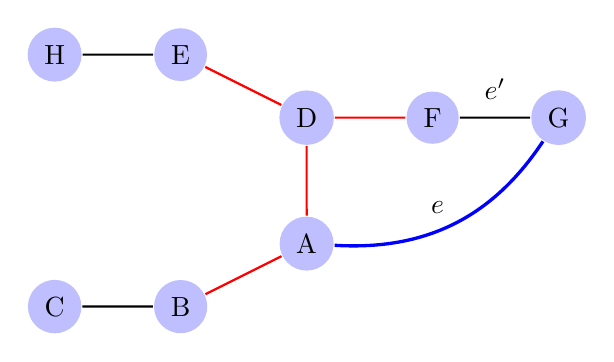
\begin{tikzpicture}
[thick,scale=.8,auto=left,every node/.style={circle,fill=blue!25}]
  \node (n6) at (4,4) {A};
  \node (n4) at (2,3) {B};
  \node (n5) at (0,3) {C};
  \node (n1) at (4,6) {D};
  \node (n2) at (2,7) {E};
  \node (n3) at (6,6) {F};
  \node (n7) at (8,6) {G};
  \node (n8) at (0,7) {H};
  \foreach \from/\to in {n5/n4,n2/n8}
    \draw (\from) -- (\to);
    
  \path[-,draw,thick,red]
  	(n4) edge (n6)
  	(n6) edge (n1)
  	(n1) edge (n2)
  	(n1) edge (n3);
  \path[-,draw,black]
  	(n3) edge node[draw=none,fill=none] {$e'$} (n7);
  \path[-,draw,very thick,blue,bend right]
  	(n6) edge node[draw=none,fill=none,color=black] {$e$} (n7);
\end{tikzpicture}